\documentclass[11pt]{article}
\usepackage[margin=1in]{geometry}
\usepackage[T1]{fontenc}
\usepackage{charter}
\usepackage{microtype}
\usepackage{amsmath}
\usepackage{graphicx}
\usepackage{booktabs}
\usepackage{tabularx}
\usepackage{longtable}
\usepackage{siunitx}
\usepackage{caption}
\usepackage[hyphens]{url}
\emergencystretch=2em
\usepackage{xcolor}
\usepackage[authoryear,round]{natbib}
\usepackage[colorlinks=true,linkcolor={black},citecolor={blue!50!black},urlcolor={blue!50!black}]{hyperref}
\captionsetup{font=small,labelfont=bf}
\graphicspath{{../outputs/figures/}}
\newcommand{\NTracts}{199}
\newcommand{\NScored}{198}
\newcommand{\PopTwenty}{585,708}
\newcommand{\PopACS}{573,243}
\newcommand{\NScenes}{39}
\newcommand{\NScenesUsed}{31}
\newcommand{\LSTmin}{35.7}
\newcommand{\LSTmax}{47.5}
\newcommand{\LSTqOne}{40.5}
\newcommand{\LSTqThree}{44.6}
\newcommand{\LSTspread}{11.8}
\newcommand{\NightMin}{18.9}
\newcommand{\NightMax}{23.0}
\newcommand{\YearCorrMin}{0.77}
\newcommand{\YearCorrMed}{0.88}
\newcommand{\DayNightRho}{0.66}
\newcommand{\PopwRho}{0.84}
\newcommand{\TreeRho}{-0.88}
\newcommand{\NDVIRho}{-0.86}
\newcommand{\OLSRtwo}{0.79}
\newcommand{\BTree}{-0.089}
\newcommand{\BTreeLo}{-0.112}
\newcommand{\BTreeHi}{-0.066}
\newcommand{\BTreeTen}{0.89}
\newcommand{\BBuilt}{0.017}
\newcommand{\BBuiltLo}{-0.003}
\newcommand{\BBuiltHi}{0.037}
\newcommand{\CompES}{0.07}
\newcommand{\CompEC}{0.39}
\newcommand{\CompSC}{0.76}
\newcommand{\PCAk}{4}
\newcommand{\PCAvar}{74}
\newcommand{\AltPCA}{0.93}
\newcommand{\AltGeo}{0.98}
\newcommand{\AltFlat}{0.91}
\newcommand{\SVIrho}{0.68}
\newcommand{\MCdraws}{1,000}
\newcommand{\RankWidth}{40}
\newcommand{\NRobust}{27}
\newcommand{\NTopTwenty}{40}
\newcommand{\StabData}{0.99}
\newcommand{\StabW}{0.98}
\newcommand{\StabBoth}{0.97}
\newcommand{\PovSlope}{0.73}
\newcommand{\PovSlopeLo}{0.44}
\newcommand{\PovSlopeHi}{1.02}
\newcommand{\RhoLSTPov}{0.32}
\newcommand{\RhoLSTBlack}{0.03}
\newcommand{\PLSTBlack}{0.71}
\newcommand{\RhoNightPov}{0.26}
\newcommand{\RhoNightBlack}{0.03}
\newcommand{\RhoHVIPov}{0.74}
\newcommand{\RhoHVIBlack}{0.53}
\newcommand{\RhoHVIInc}{-0.72}
\newcommand{\ExpDayAll}{41.97}
\newcommand{\ExpDayBlack}{41.96}
\newcommand{\ExpDayWhite}{41.91}
\newcommand{\ExpDayHisp}{42.11}
\newcommand{\ExpDayPov}{42.49}
\newcommand{\ExpDayOld}{41.68}
\newcommand{\ExpNightAll}{21.00}
\newcommand{\ExpNightBlack}{20.99}
\newcommand{\ExpNightWhite}{20.98}
\newcommand{\ExpNightHisp}{21.17}
\newcommand{\ExpNightPov}{21.11}
\newcommand{\ExpNightOld}{20.91}
\newcommand{\HolcA}{40.7}
\newcommand{\HolcB}{40.2}
\newcommand{\HolcC}{43.8}
\newcommand{\HolcD}{44.7}
\newcommand{\HolcDminusAB}{4.4}
\newcommand{\HolcTreeA}{44}
\newcommand{\HolcTreeB}{47}
\newcommand{\HolcTreeC}{18}
\newcommand{\HolcTreeD}{8}
\newcommand{\HolcNA}{9}
\newcommand{\HolcNB}{38}
\newcommand{\HolcNC}{44}
\newcommand{\HolcND}{46}
\newcommand{\HolcKW}{69.6}
\newcommand{\HolcSlope}{2.07}
\newcommand{\HolcSlopeLo}{1.72}
\newcommand{\HolcSlopeHi}{2.41}
\newcommand{\HolcNightD}{21.9}
\newcommand{\HolcNightB}{20.5}
\newcommand{\MoranHVI}{0.71}
\newcommand{\MoranLST}{0.75}
\newcommand{\MoranNight}{0.88}
\newcommand{\MoranSens}{0.55}
\newcommand{\MoranCap}{0.56}
\newcommand{\LisaHH}{45}
\newcommand{\LisaLL}{48}
\newcommand{\LisaHL}{1}
\newcommand{\LisaHHpop}{90,735}
\newcommand{\VHn}{40}
\newcommand{\VHpop}{78,314}
\newcommand{\VHdist}{1.08}
\newcommand{\AllDist}{1.39}
\newcommand{\NCool}{29}
\newcommand{\NZcta}{20}
\newcommand{\ValHVI}{0.69}
\newcommand{\ValHVIp}{$<$0.001}
\newcommand{\ValHVIlo}{0.35}
\newcommand{\ValHVIhi}{0.89}
\newcommand{\ValLST}{0.79}
\newcommand{\ValLSTp}{$<$0.001}
\newcommand{\ValNight}{0.66}
\newcommand{\ValNightp}{0.001}
\newcommand{\ValExp}{0.72}
\newcommand{\ValExpp}{$<$0.001}
\newcommand{\ValSens}{0.14}
\newcommand{\ValSensp}{0.543}
\newcommand{\ValCap}{0.61}
\newcommand{\ValCapp}{0.004}
\newcommand{\ValSVI}{0.27}
\newcommand{\ValSVIp}{0.247}
\newcommand{\ValHHI}{0.59}
\newcommand{\ValHHIp}{0.006}
\newcommand{\ExcessRtwo}{0.56}
\newcommand{\ExcessAdjExp}{0.53}
\newcommand{\FullRtwo}{0.78}
\newcommand{\FullAdj}{0.74}
\newcommand{\NestedF}{7.9}
\newcommand{\NestedFp}{0.004}
\newcommand{\LooFull}{6.4}
\newcommand{\LooExp}{8.2}
\newcommand{\CapCoef}{284}
\newcommand{\CapCoefLo}{129}
\newcommand{\CapCoefHi}{439}
\newcommand{\SensCoef}{-131}
\newcommand{\SensCoefLo}{-210}
\newcommand{\SensCoefHi}{-52}
\newcommand{\DMHtmin}{4.8}
\newcommand{\DMHtmax}{1.6}
\newcommand{\DMHtminC}{2.7}
\newcommand{\DMHtmaxC}{0.9}
\newcommand{\PairedDays}{380}
\newcommand{\BWInightsTwentyFive}{11}
\newcommand{\DMHnightsTwentyFive}{42}
\newcommand{\BWIdaysTwentyFive}{28}
\newcommand{\DMHdaysTwentyFive}{58}
\newcommand{\VHLST}{44.8}
\newcommand{\RestLST}{41.5}
\newcommand{\VHNight}{22.0}
\newcommand{\RestNight}{20.8}
\newcommand{\VHPov}{34}
\newcommand{\RestPov}{18}
\newcommand{\VHCHD}{9.2}
\newcommand{\RestCHD}{6.1}
\newcommand{\VHTree}{13}
\newcommand{\RestTree}{34}
\newcommand{\VHBlack}{84}
\newcommand{\RestBlack}{55}
\newcommand{\VHNoVeh}{48}
\newcommand{\RestNoVeh}{23}
\newcommand{\VHShut}{27}
\newcommand{\RestShut}{14}
\newcommand{\TopCSAone}{Sandtown-Winchester/Harlem Park}
\newcommand{\TopCSAtwo}{Southwest Baltimore}
\newcommand{\TopCSAthree}{Clifton-Berea}
\newcommand{\NHotQ}{50}
\newcommand{\NHotWhite}{12}

\newcommand{\degC}{\,\textdegree C}

\title{\textbf{Where Heat Meets Vulnerability:\\ A Validated, Uncertainty-Aware Heat Vulnerability Index for Baltimore City's Census Tracts}}
\author{Sahil\\[2pt]\small MSE in Data Science, Whiting School of Engineering, Johns Hopkins University, Baltimore, MD\\\small \texttt{sfnu1@jh.edu}}
\date{October 2026}

\begin{document}
\maketitle

\begin{abstract}
\noindent Extreme heat is the leading weather-related cause of death in the United States, and its burden is uneven within cities. We build a tract-level Heat Vulnerability Index (HVI) for Baltimore City, Maryland, from the most recent public data available in October 2026, and we test it against an independent health outcome. Exposure combines a population-weighted daytime land surface temperature (LST) composite from \NScenesUsed{} cloud-screened Landsat~8/9 summer scenes (2019--2025, 30\,m) with night-time LST from MODIS Aqua (about 01:30 local solar time). Sensitivity combines age and seven model-based chronic-condition and disability measures (CDC PLACES 2025; ACS 2020--2024). Low adaptive capacity combines ten indicators covering poverty, mobility, isolation, language, insurance, connectivity, utility shut-off risk, housing age, cooling-centre access and tree cover. Across \NScored{} populated tracts, mean daytime LST where people live ranged from \LSTmin{} to \LSTmax\degC{}. Tree cover explained most of this gradient (Spearman $\rho=\TreeRho$), and tracts graded ``D'' by the 1937 HOLC redlining maps were \HolcDminusAB\degC{} hotter than those graded A or B. Vulnerability was strongly clustered (Moran's $I=\MoranHVI$), with \LisaHH{} tracts forming two contiguous hot spots in East and West Baltimore. A Monte Carlo analysis propagating ACS margins of error, PLACES confidence intervals, inter-annual LST variation and random component weights left the ranking highly stable (median Spearman $\rho=\StabBoth$ against the baseline). \NRobust{} tracts fell in the top 20\% in at least 90\% of \MCdraws{} draws. Aggregated to \NZcta{} ZIP code areas, the HVI tracked heat-related EMS activations for 2020--2022 ($\rho=\ValHVI$, 95\% bootstrap CI \ValHVIlo--\ValHVIhi). The CDC/ATSDR Social Vulnerability Index did not ($\rho=\ValSVI$). Low adaptive capacity explained variation in EMS activations beyond exposure (nested $F=\NestedF$, $p=\NestedFp$). Daytime heat exposure was not associated with tract racial composition but was associated with poverty. Vulnerability, however, was strongly patterned by both. All data, code, figures and an interactive dashboard are released for reuse.

\medskip\noindent\textbf{Keywords:} urban heat; heat vulnerability index; land surface temperature; Landsat; MODIS; CDC PLACES; redlining; environmental justice; spatial statistics; Baltimore
\end{abstract}

\section{Introduction}

Over the 30-year record kept by the National Weather Service, excessive heat has caused more deaths than any other weather hazard in the United States \citep{nws}. Heat risk is also highly local. Within one city, tree-lined neighbourhoods and blocks of rowhouses, flat roofs and asphalt can differ in surface temperature by more than ten degrees on the same summer morning. The people living in those places differ too, in age, health and the resources they have to cope.

Baltimore shows both forms of inequality clearly. Across 108 U.S. urban areas, \citet{hoffman2020} found that neighbourhoods graded ``hazardous'' (D) on the 1930s Home Owners' Loan Corporation (HOLC) maps are hotter today. Baltimore's formerly redlined areas were about 3.2\degC{} warmer than the city-wide average, among the largest anomalies in their sample. \citet{huang2011} linked Baltimore's Landsat surface temperatures to land cover and neighbourhood socioeconomic status. \citet{corpuz2026} showed that night-time heat waves were followed by more asthma emergency department visits in Baltimore, and that neighbourhood-scale temperature predicted those visits better than the airport station.

Heat vulnerability indices (HVIs) translate these patterns into a ranking that health departments can use. The reference design is \citet{reid2009}: ten census variables reduced by principal components and summed. Most later indices follow the IPCC framing of vulnerability as a function of exposure, sensitivity and adaptive capacity \citep{ipcc2007}. Three weaknesses are common. Indices are rarely tested against health outcomes inside a single city. They rarely report how uncertain their rankings are. And they often use exposure data from a single satellite overpass or none at all.

This study addresses all three for Baltimore City. We ask: \emph{Where in Baltimore do heat exposure, physiological sensitivity and low adaptive capacity coincide? How certain is that ranking? Does it track real heat-related health harm?} We make four contributions:
\begin{enumerate}
  \item \textbf{Current, fine-grained inputs.} We use the latest releases available in October 2026 (ACS 2020--2024, CDC PLACES 2025, SVI 2022, 2026 cooling-centre locations). Exposure is built from seven summers of Landsat imagery at 30\,m, weighted by where people actually live (2020 census blocks), plus night-time MODIS temperatures.
  \item \textbf{Quantified uncertainty.} We propagate survey error, model error, inter-annual temperature variation and weighting choices through \MCdraws{} Monte Carlo draws and report a rank interval and a top-20\% probability for every tract.
  \item \textbf{External validation.} We test the index against heat-related EMS activations reported to NEMSIS for 2020--2022, an outcome not used to build it, and compare it with the CDC/ATSDR SVI and the CDC Heat \& Health Index.
  \item \textbf{Mechanism and equity.} We quantify the role of tree cover, the persistence of the redlining signal, and how exposure and vulnerability are distributed by race and income.
\end{enumerate}

\section{Data}

All inputs are public. Table~\ref{tab:data} lists them. Because several federal download endpoints were not reachable from the analysis environment, every file was retrieved from its official API or download page through a standard web browser. The scripts record each request.

\begin{table}[ht]\centering\small
\caption{Data sources (all accessed 21 October 2026).}\label{tab:data}
\begin{tabularx}{\textwidth}{@{}l X l@{}}\toprule
Domain & Dataset & Resolution / vintage \\\midrule
Boundaries & 2020 census tracts, blocks (with 2020 population) and ZCTAs, TIGERweb \citep{tigerweb} & \NTracts{} tracts; 10,025 blocks \\
Day heat & Landsat 8/9 Collection 2 Level-2 surface temperature, red and NIR bands \citep{usgs_l89}, via Planetary Computer \citep{pc} & 30\,m; \NScenesUsed{} of \NScenes{} summer scenes, 2019--25 \\
Night heat & MODIS Aqua/Terra MYD11A2/MOD11A2 v061 8-day LST \citep{myd11a2} & 1\,km; Jun--Aug 2019--25 \\
Land cover & ESA WorldCover 2021 v200 \citep{worldcover} & 10\,m \\
Health & CDC PLACES, census tract, 2025 release \citep{places2025,zhang2014,zhang2015} & BRFSS 2023 (most measures) \\
Social & American Community Survey 5-year, 18 tables with margins of error \citep{acs2024} & 2020--2024 \\
Social & CDC/ATSDR Social Vulnerability Index \citep{flanagan2011,svi2022} & 2022, Maryland-ranked \\
Services & Baltimore City cooling centres \citep{baltcool} & \NCool{} sites, 2026 \\
History & Mapping Inequality HOLC areas, 2020-tract crosswalk \citep{mappingineq} & 1937 map \\
Outcome & CDC/ATSDR Heat \& Health Index: percentile of heat-related EMS activation rate (NEMSIS) \citep{hhi2024} & ZCTA; 2020--22 \\
Climate & Daily Tmax/Tmin, BWI airport and Inner Harbor (DMH) \citep{acis} & 2019--2025 \\
Names & Community Statistical Areas \citep{bnia} & 56 CSAs \\\bottomrule
\end{tabularx}
\end{table}

\section{Methods}

\subsection{Heat exposure}
For each Landsat scene we masked fill, dilated cloud, cirrus, cloud, cloud shadow and water using the QA\_PIXEL band (bits 1--4 and 7). We converted digital numbers to temperature as $T = 0.00341802\,\mathrm{DN} + 149.0 - 273.15$ (\textdegree C). Undetected cloud and haze were removed by discarding pixels colder than both 15\degC{} and the scene median minus 15\degC. Scenes with less than 30\% clear land were dropped, leaving \NScenesUsed{} of \NScenes{} scenes. These scenes give a median of 24 clear observations per pixel. The per-pixel median across all scenes gives a typical clear-sky summer morning surface (Landsat 8/9 image Baltimore at about 11:45 a.m.\ Eastern Daylight Time).

We then weighted this surface by population. Each of Baltimore's 2020 census blocks takes the mean LST of the $3\times3$ pixel window (90\,m) around its internal point. A tract's exposure is the block-population-weighted mean of these values, so parks and industrial land inside a tract do not dilute the temperature its residents experience. Night-time exposure is the per-cell median of all quality-screened MODIS Aqua 8-day night composites (overpass about 01:30 local solar time) for June--August 2019--2025. These were resampled to the same 30\,m grid and averaged by tract.

\subsection{Indicators and index}
Table~\ref{tab:ind} lists the 21 indicators, grouped into exposure (2), sensitivity (9) and low adaptive capacity (10). We used shares rather than counts, and oriented every indicator so that a higher value means more vulnerable. We added three indicators that most HVIs omit:
\begin{itemize}
  \item the PLACES estimate of adults threatened with a utility shut-off in the past year, a direct proxy for inability to run air conditioning;
  \item population-weighted distance to the nearest 2026 cooling centre;
  \item the absence of tree cover.
\end{itemize}
Among the \NScored{} tracts with at least 100 residents, each indicator was converted to a within-city percentile rank. Component scores are the mean percentile of their indicators. The HVI is the equal-weight mean of the three components:
\begin{equation}
\mathrm{HVI}_i = \tfrac13\left(E_i + S_i + C_i\right), \qquad E_i,\,S_i,\,C_i = \frac{1}{|K|}\sum_{k\in K} \frac{\operatorname{rank}(x_{ik})}{n}.
\end{equation}
Tracts were grouped into quintiles for mapping.

\subsection{Uncertainty and robustness}
We ran \MCdraws{} Monte Carlo draws. Each draw perturbed every ACS share by $\mathcal N(0,\mathrm{MOE}/1.645)$, using Census Bureau formulas for derived proportions \citep{acsguide}. It perturbed every PLACES estimate by $\mathcal N(0,\mathrm{SE})$, with SE recovered from the 95\% interval. It perturbed daytime LST by the standard error of its seven annual tract anomalies. Finally, it drew component weights from a Dirichlet(4,4,4) distribution. For each tract we report the 5th--95th percentile of its rank and the probability that it ranks in the top 20\%. We also compared the HVI with three alternative constructions: a principal components index in the style of \citet{reid2009}, a geometric mean of components, and a flat mean of all 21 indicators.

\subsection{Spatial structure, drivers and equity}
Global Moran's $I$ \citep{moran1950} and Local Moran's $I$ \citep{anselin1995} used row-standardised Queen contiguity with 999 permutations. Drivers of daytime heat were estimated by OLS of tract LST on tree and built-up cover, with HC3 standard errors. Group-level exposure was computed as the population-weighted mean LST experienced by members of each ACS group. HOLC grades were assigned when at least 50\% of a tract's area was graded, using the dominant grade.

\subsection{Validation against health outcomes}
Tract-level heat illness counts are not public. We therefore aggregated tract scores to ZCTAs using 2020 block populations and compared them with the HHI percentile rank of the heat-related EMS activation rate per 100,000 residents (NEMSIS, 2020--2022 average). We kept ZCTAs with at least 5,000 Baltimore City residents, at least 50\% of their population inside the city, and no low-count flag, giving \NZcta. We report Spearman correlations with 2,000-draw bootstrap intervals. We then asked whether sensitivity and capacity explain EMS activity beyond exposure, using a nested $F$-test and leave-one-out prediction error.

\section{Results}

\subsection{Exposure}
Daytime surface temperature where people live ranged from \LSTmin\degC{} to \LSTmax\degC{} across tracts, with an interquartile range of \LSTqOne--\LSTqThree\degC. Night-time surface temperature ranged from \NightMin{} to \NightMax\degC{} (Figure~\ref{fig:lst}). The pattern was stable over time: tract rankings in individual summers correlated with each other at a median $\rho$ of \YearCorrMed{} (minimum \YearCorrMin). Day and night exposure were related but distinct ($\rho=\DayNightRho$): night-time heat was highest in the dense rowhouse neighbourhoods of East Baltimore (Clifton-Berea, Oldtown/Middle East, Madison/East End) and the southeastern harbour district (Figure~\ref{fig:lst}b). Weather stations confirm a strong night-time urban heat island. On \PairedDays{} paired summer days, the Inner Harbor station recorded minimum temperatures \DMHtmin\,\textdegree F (\DMHtminC\degC) warmer than BWI airport, but maximum temperatures only \DMHtmax\,\textdegree F warmer. In summer 2025, the Inner Harbor recorded \DMHnightsTwentyFive{} nights at or above 75\,\textdegree F, against \BWInightsTwentyFive{} at BWI (Figure~\ref{fig:station}).

\begin{figure}[ht]\centering
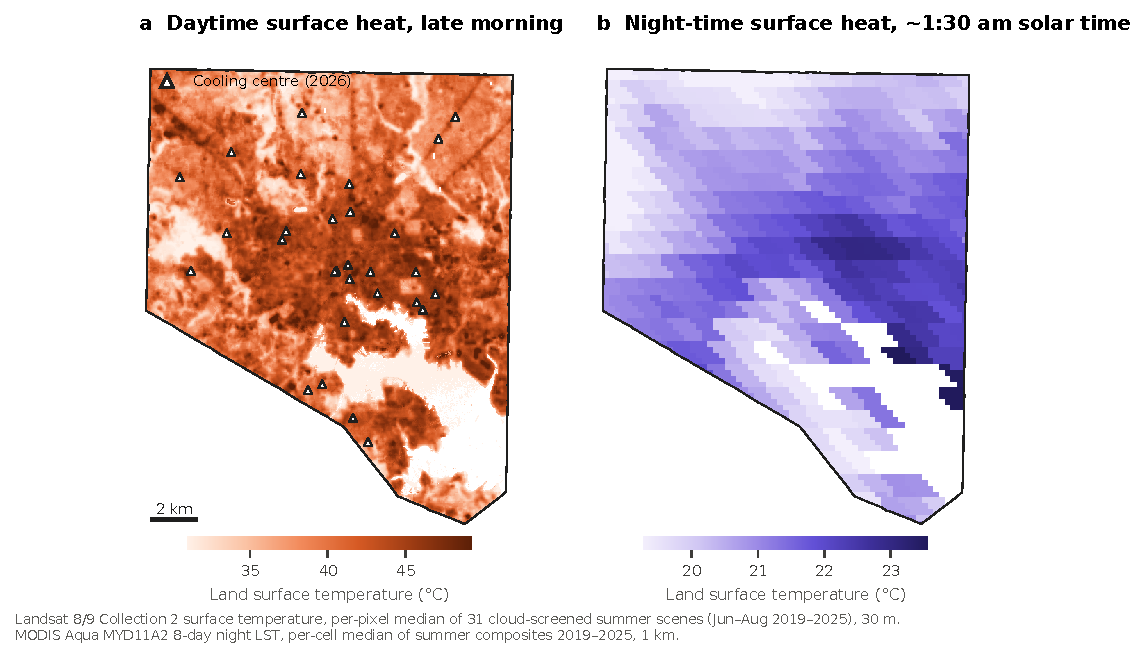
\includegraphics[width=\textwidth]{fig1_lst_day_night.pdf}
\caption{Summer land surface temperature, Baltimore City. (a) Landsat 30\,m median of \NScenesUsed{} cloud-screened scenes, 2019--2025, with 2026 cooling centres. (b) MODIS Aqua night-time LST, 1\,km.}\label{fig:lst}
\end{figure}

Tree cover was the dominant correlate of surface heat ($\rho=\TreeRho$; NDVI $\rho=\NDVIRho$). In a joint model, tree and built-up cover explained $R^2=\OLSRtwo$ of the variation in tract LST. Each additional 10 percentage points of tree cover was associated with \BTreeTen\degC{} lower surface temperature (95\% CI \BTreeLo{} to \BTreeHi{} per point). Once trees were accounted for, built-up share added little (\BBuilt, CI \BBuiltLo{} to \BBuiltHi; Figure~\ref{fig:drivers}).

\subsection{The Heat Vulnerability Index}
The three components measure different things. Exposure was nearly unrelated to sensitivity ($\rho=\CompES$) and moderately related to low capacity ($\rho=\CompEC$), while sensitivity and low capacity were closely related ($\rho=\CompSC$; Figure~\ref{fig:comp}). The HVI correlated with the SVI at $\rho=\SVIrho$, so it shares a social core with the SVI but is not the same measure.

The \VHn{} tracts in the very-high quintile are home to \VHpop{} people. Compared with the rest of the city, measured as population-weighted means, they are:
\begin{itemize}
  \item hotter by day and by night (\VHLST{} vs \RestLST\degC; \VHNight{} vs \RestNight\degC);
  \item poorer (\VHPov\% vs \RestPov\% below the poverty line);
  \item sicker (coronary heart disease \VHCHD\% vs \RestCHD\%);
  \item less treed (\VHTree\% vs \RestTree\% tree cover);
  \item more often without a car (\VHNoVeh\% vs \RestNoVeh\% of households);
  \item more often under threat of a utility shut-off (\VHShut\% vs \RestShut\% of adults).
\end{itemize}
They are concentrated in \TopCSAone, \TopCSAtwo{} and \TopCSAthree{} (Table~\ref{tab:top}, Figure~\ref{fig:hvi}).

\begin{figure}[ht]\centering
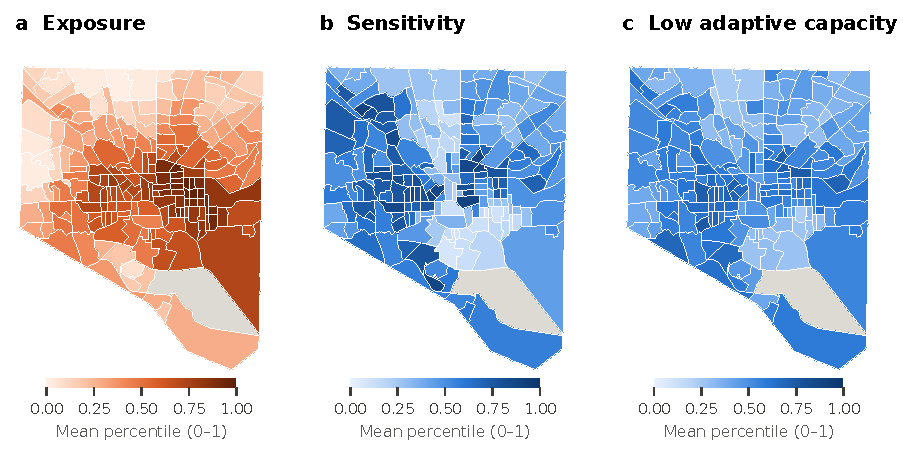
\includegraphics[width=\textwidth]{fig2_components.pdf}
\caption{Component scores (mean within-city percentile of each component's indicators). Grey: tract with fewer than 100 residents.}\label{fig:comp}
\end{figure}

\begin{figure}[ht]\centering
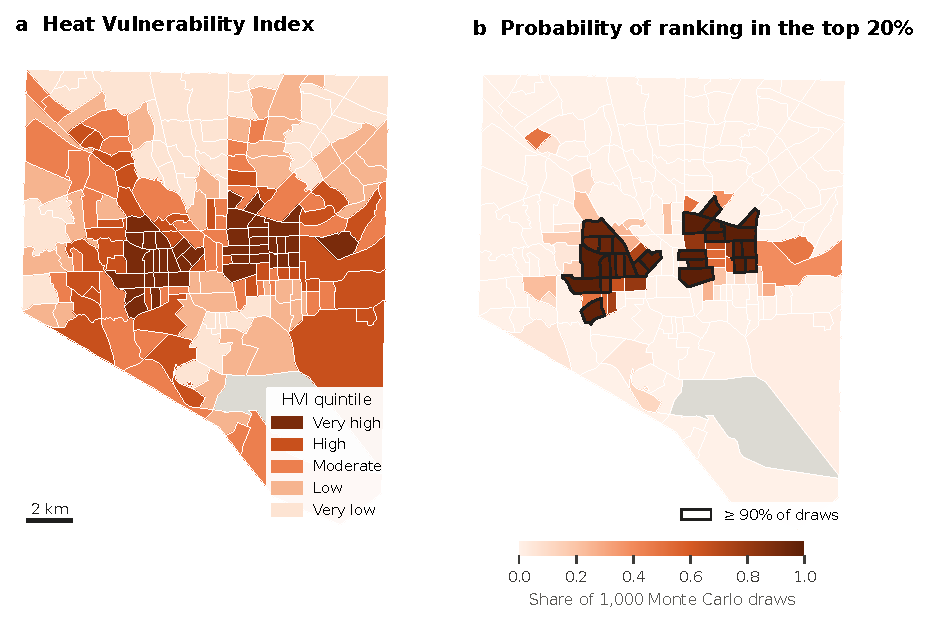
\includegraphics[width=\textwidth]{fig3_hvi_uncertainty.pdf}
\caption{(a) Heat Vulnerability Index quintiles. (b) Probability that each tract ranks in the top 20\% across \MCdraws{} Monte Carlo draws that perturb data error, inter-annual LST and component weights. Outlined: probability $\ge 0.9$.}\label{fig:hvi}
\end{figure}

\subsection{How certain is the ranking?}
The ranking was robust. Across Monte Carlo draws, the median Spearman correlation with the baseline ranking was \StabData{} when only data error varied, \StabW{} when only weights varied, and \StabBoth{} when both varied. Of the \NTopTwenty{} tracts in the top 20\%, \NRobust{} stayed there in at least 90\% of draws (Figure~\ref{fig:hvi}b). The median 90\% rank interval spanned \RankWidth{} places. Uncertainty is therefore real for middle-ranked tracts but small at the top (Figure~\ref{fig:rank}). The alternative constructions agreed closely with the baseline: $\rho=\AltPCA$ for the PCA index (\PCAk{} components, \PCAvar\% of variance), \AltGeo{} for the geometric mean and \AltFlat{} for the flat mean.

\begin{table}[ht]\centering\footnotesize
\setlength{\tabcolsep}{3.5pt}
\caption{The 15 highest-ranked tracts. Rank interval: 5th--95th percentile across Monte Carlo draws. $P_{20}$: probability of ranking in the top 20\%. LST: population-weighted daytime; Night: MODIS night-time (\textdegree C). Poverty, CHD and tree cover in \%.}\label{tab:top}
\begin{tabular}{@{}rlllcccccccc@{}}\toprule
Rank & Tract & Community Statistical Area & HVI & 90\% interval & $P_{20}$ & LST & Night & Pov. & CHD & Tree \\\midrule
1 & 805 & Clifton-Berea & 0.852 & 1--2 & 1.00 & 46.8 & 22.5 & 52 & 12.2 & 8 \\
2 & 803.01 & Clifton-Berea & 0.803 & 2--17 & 1.00 & 46.4 & 23.0 & 25 & 9.1 & 8 \\
3 & 908 & Midway/Coldstream & 0.795 & 2--16 & 1.00 & 46.4 & 22.1 & 26 & 11.1 & 11 \\
4 & 702 & Madison/East End & 0.781 & 2--24 & 1.00 & 47.5 & 22.8 & 34 & 8.1 & 3 \\
5 & 1002 & Oldtown/Middle East & 0.779 & 3--19 & 1.00 & 45.5 & 22.4 & 48 & 10.3 & 10 \\
6 & 806 & Oliver/Johnston Square & 0.767 & 3--23 & 1.00 & 45.8 & 22.4 & 23 & 10.0 & 5 \\
7 & 802 & Clifton-Berea & 0.766 & 2--22 & 1.00 & 44.0 & 22.5 & 46 & 11.6 & 8 \\
8 & 2805 & Oldtown/Middle East & 0.765 & 2--19 & 1.00 & 45.4 & 21.9 & 67 & 13.1 & 2 \\
9 & 907 & Midway/Coldstream & 0.764 & 3--28 & 0.99 & 44.2 & 21.7 & 36 & 10.9 & 15 \\
10 & 803.02 & Clifton-Berea & 0.758 & 4--28 & 0.99 & 45.0 & 22.9 & 31 & 7.9 & 4 \\
11 & 1001 & Oliver/Johnston Square & 0.754 & 4--23 & 1.00 & 44.8 & 22.5 & 34 & 9.0 & 9 \\
12 & 1603 & Sandtown-Winchester/Harlem Park & 0.748 & 3--36 & 0.98 & 43.3 & 21.9 & 41 & 11.8 & 22 \\
13 & 2002 & Southwest Baltimore & 0.746 & 3--25 & 1.00 & 44.8 & 21.6 & 39 & 13.2 & 16 \\
14 & 1702 & Upton/Druid Heights & 0.744 & 4--26 & 1.00 & 43.8 & 22.0 & 61 & 10.9 & 6 \\
15 & 1605 & Greater Rosemont & 0.733 & 6--27 & 1.00 & 45.0 & 21.4 & 32 & 10.3 & 22 \\

\bottomrule\end{tabular}
\end{table}

\subsection{Spatial clustering}
Vulnerability was strongly clustered (Moran's $I=\MoranHVI$, $p=0.001$), as were daytime LST (\MoranLST), night-time LST (\MoranNight), sensitivity (\MoranSens) and low capacity (\MoranCap). Local Moran's $I$ identified \LisaHH{} high--high tracts, home to \LisaHHpop{} residents. They form two contiguous clusters, one in West Baltimore and one in East Baltimore. \LisaLL{} low--low tracts form a northern band and a smaller cluster south of the Inner Harbor (Figure~\ref{fig:lisa}).

\begin{figure}[ht]\centering
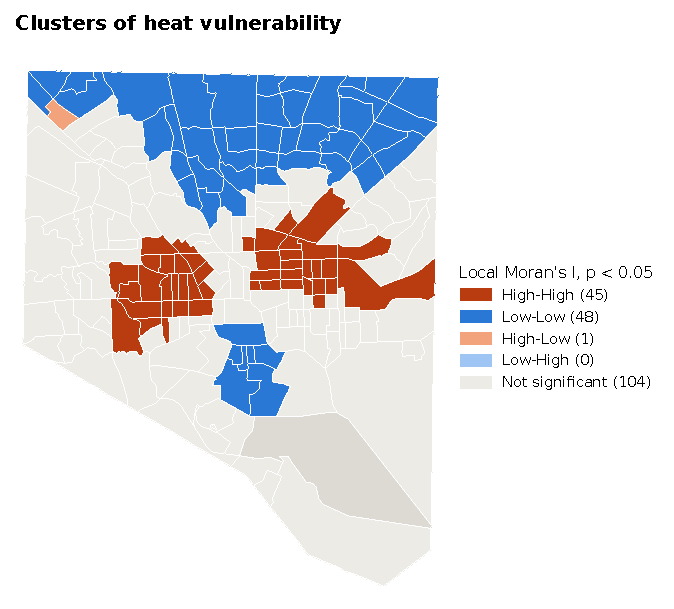
\includegraphics[width=0.78\textwidth]{fig4_lisa.pdf}
\caption{Local indicators of spatial association for the HVI (Queen contiguity, 999 permutations, $p<0.05$).}\label{fig:lisa}
\end{figure}

\subsection{Redlining, race and income}
Among tracts mostly covered by the 1937 HOLC map, mean daytime LST rose from \HolcA\degC{} (A, $n=\HolcNA$) and \HolcB\degC{} (B, $n=\HolcNB$) to \HolcC\degC{} (C, $n=\HolcNC$) and \HolcD\degC{} (D, $n=\HolcND$). The difference across grades was significant (Kruskal--Wallis $H=\HolcKW$, $p<0.001$). Each step down the HOLC scale was associated with \HolcSlope\degC{} more surface heat (95\% CI \HolcSlopeLo--\HolcSlopeHi). Tree cover told the same story in reverse: \HolcTreeA\% and \HolcTreeB\% in A and B areas, against \HolcTreeC\% and \HolcTreeD\% in C and D areas (Figure~\ref{fig:holc}).

Exposure and vulnerability were patterned differently.
\begin{itemize}
  \item \textbf{Exposure followed poverty.} Daytime LST rose with tract poverty ($\rho=\RhoLSTPov$; \PovSlope\degC{} per 10 percentage points, CI \PovSlopeLo--\PovSlopeHi).
  \item \textbf{Exposure did not follow race.} Daytime LST was not associated with the share of non-Hispanic Black residents ($\rho=\RhoLSTBlack$, $p=\PLSTBlack$). Population-weighted daytime exposure was nearly identical for Black (\ExpDayBlack\degC) and white (\ExpDayWhite\degC) residents, and slightly higher for residents below poverty (\ExpDayPov\degC). \NHotWhite{} of the \NHotQ{} hottest tracts (top quartile) are majority non-Hispanic white, low-poverty rowhouse neighbourhoods around the harbour (Canton, Federal Hill, Fells Point, Highlandtown, South Baltimore). They offset hot, majority-Black districts in East and West Baltimore.
  \item \textbf{Vulnerability followed both.} The HVI was strongly associated with poverty ($\rho=\RhoHVIPov$) and with the Black population share ($\rho=\RhoHVIBlack$). Residents of very-high tracts are \VHBlack\% non-Hispanic Black, against \RestBlack\% elsewhere.
\end{itemize}
In Baltimore, then, the racial disparity in heat risk works mainly through sensitivity and adaptive capacity rather than through surface temperature alone.

\begin{figure}[ht]\centering
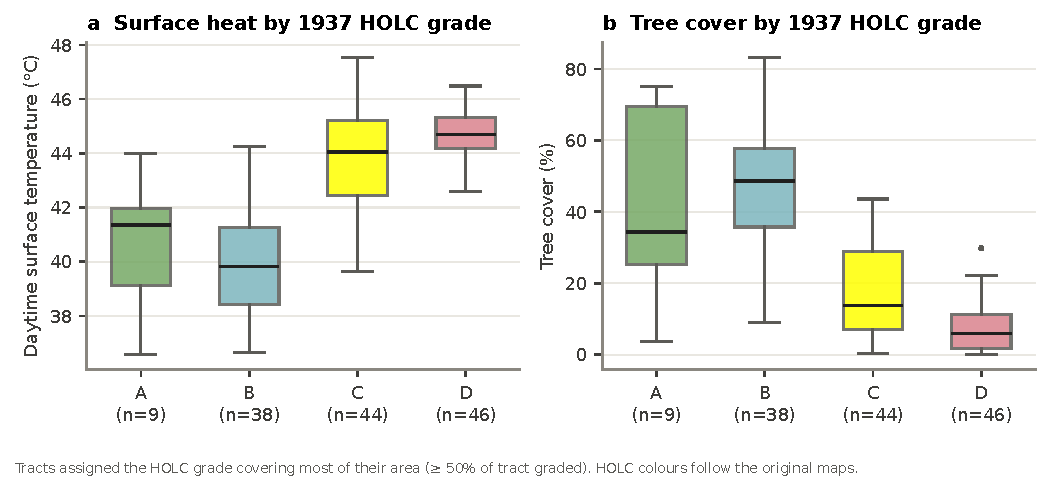
\includegraphics[width=0.95\textwidth]{fig5_holc.pdf}
\caption{Daytime surface temperature and tree cover by 1937 HOLC grade.}\label{fig:holc}
\end{figure}

\subsection{Validation against heat-related EMS activations}
At ZCTA level, the HVI was positively associated with the heat-related EMS activation percentile ($\rho=\ValHVI$, $p=\ValHVIp$; bootstrap 95\% CI \ValHVIlo--\ValHVIhi; Table~\ref{tab:val}, Figure~\ref{fig:val}). So were the exposure component (\ValExp) and the low-capacity component (\ValCap). The sensitivity component alone was not (\ValSens). Daytime LST alone correlated at \ValLST. The SVI did not track EMS activity ($\rho=\ValSVI$, $p=\ValSVIp$), while the national HHI did ($\rho=\ValHHI$).

\begin{table}[ht]\centering\small
\caption{Spearman correlation with the heat-related EMS activation percentile (NEMSIS 2020--2022, via CDC HHI), \NZcta{} Baltimore ZCTAs.}\label{tab:val}
\begin{tabular}{@{}lcc@{}}\toprule
Measure (ZCTA, population-weighted) & $\rho$ & $p$ \\\midrule
Heat Vulnerability Index (this study) & 0.69 & $<$0.001 \\
\quad Exposure component & 0.72 & $<$0.001 \\
\quad Sensitivity component & 0.14 & 0.543 \\
\quad Low-capacity component & 0.61 & 0.004 \\
Daytime LST alone & 0.79 & $<$0.001 \\
Night-time LST alone & 0.66 & 0.001 \\
CDC/ATSDR SVI 2022 & 0.27 & 0.247 \\
CDC Heat \& Health Index 2024 (overall) & 0.59 & 0.006 \\

\bottomrule\end{tabular}
\end{table}

\begin{figure}[ht]\centering
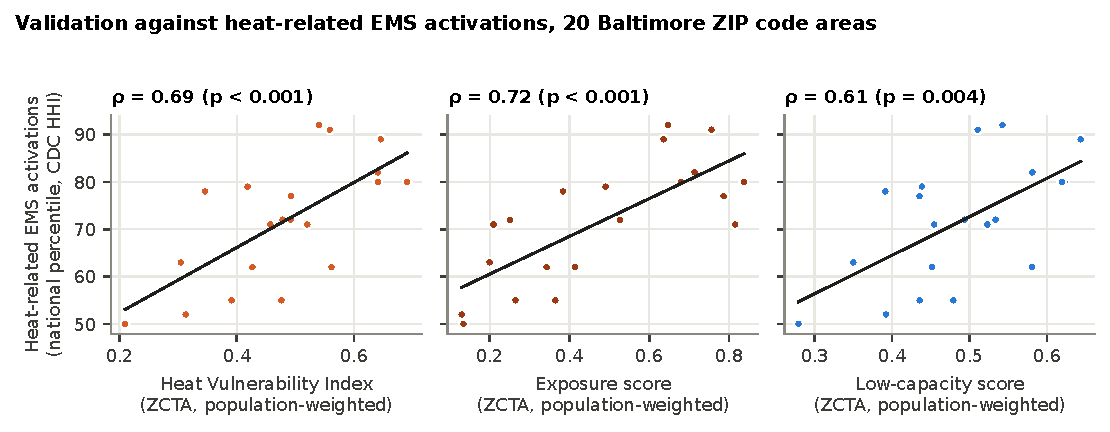
\includegraphics[width=\textwidth]{fig7_validation.pdf}
\caption{ZCTA-level validation against heat-related EMS activations. Lines are least-squares fits.}\label{fig:val}
\end{figure}

\paragraph{Harm beyond exposure.} Exposure alone explained $R^2=\ExcessRtwo$ of the variation in EMS activity across ZCTAs (adjusted \ExcessAdjExp). Adding sensitivity and capacity raised this to $R^2=\FullRtwo$ (adjusted \FullAdj; nested $F=\NestedF$, $p=\NestedFp$). Leave-one-out prediction error fell from \LooExp{} to \LooFull{} percentile points. Low capacity carried the added signal (coefficient \CapCoef, 95\% CI \CapCoefLo{} to \CapCoefHi). The sensitivity coefficient became negative once low capacity was included. This is consistent with the strong collinearity between the two ($\rho=\CompSC$) in a sample of \NZcta, and should not be read as a protective effect. Where heat sends people to EMS beyond what temperature predicts, the evidence points to limited resources to cope rather than to chronic-disease prevalence alone.

\section{Discussion}

\paragraph{What the index adds.} The HVI is built from the most recent public data, carries a stated uncertainty for every tract, and tracks an independent outcome at the scale where one is available. Three findings matter most for practice.
\begin{enumerate}
  \item \textbf{Concentrated, predictable risk.} Risk is concentrated in two contiguous areas in East and West Baltimore. Their ranking is stable across survey error, model error, inter-annual temperature variation and analyst choices of weights.
  \item \textbf{Capacity, not disease, explains excess harm.} Adaptive capacity, more than disease prevalence, explains why some places see more heat-related EMS activity than their temperature predicts. Interventions that restore the ability to cool (utility shut-off protection, cooling assistance, transport to cooling centres, wellness checks for older adults living alone) target that gap directly.
  \item \textbf{Trees close the exposure gap.} Tree cover is the dominant, and modifiable, driver of the daytime surface gradient. The roughly \BTreeTen\degC{} association per 10 points of canopy, together with the \HolcDminusAB\degC{} D-versus-A/B redlining gap and the corresponding canopy gap, gives a quantitative target for canopy equity programmes.
\end{enumerate}

\paragraph{Cooling-centre access.} The \NCool{} cooling centres open in 2026 are, on average, closer to residents of very-high tracts (\VHdist\,km, population-weighted straight-line distance) than to the city as a whole (\AllDist\,km). Siting already tracks need. The binding constraint is more likely getting there, given that \VHNoVeh\% of households in these tracts have no car, and being able to stay cool at home at night.

\paragraph{Comparison with national tools.} The SVI is widely used for heat planning, but it did not track heat-related EMS activity in Baltimore. A heat-specific, locally ranked index did. This supports building purpose-specific indices rather than reusing general social vulnerability scores.

\section{Scope and robustness}
We designed the study to close the usual weaknesses of HVIs. A few conditions remain inherent to the public data, and we state them with how each was handled.
\begin{itemize}
  \item \textbf{Surface versus air temperature.} Satellites measure surfaces, not the air people breathe. We addressed this by using seven summers (not one scene), weighting by where people live, adding night-time MODIS temperatures, and checking against two weather stations. Street-level air temperature campaigns (NOAA Heat Watch, 2018) would add resolution; the public service hosting them was offline during this study.
  \item \textbf{Outcome resolution.} Heat-illness counts are not released below ZIP code level. Validation is therefore at ZCTA scale ($n=\NZcta$), with bootstrap intervals and leave-one-out checks.
  \item \textbf{Modelled health data.} PLACES values are small-area estimates. Their stated uncertainty is carried through the Monte Carlo analysis.
  \item \textbf{Ecological design.} All measures describe places, not individuals, and the associations are not causal estimates.
\end{itemize}

\section{Conclusion}
Baltimore's heat risk is concentrated, persistent and measurable. Combining seven summers of satellite temperature with the most recent health and social data produces a tract ranking that is robust to its uncertainties and tracks heat-related EMS activity. The tracts it identifies match the city's redlining history and its tree-canopy gaps. The index, data and interactive dashboard are released so that the ranking can be updated as new data arrive and used to target cooling, canopy and outreach where they are needed most.

\section*{Data and code availability}
All inputs are public (Table~\ref{tab:data}). Python scripts reproduce every number, table and figure: \texttt{01\_landsat.py} through \texttt{06\_tex\_tables.py}. Every value quoted in this paper is written automatically from \texttt{results.json} into \texttt{macros.tex}. The tract-level dataset and an interactive dashboard accompany the paper.

\section*{Acknowledgements}
Tree-cover classes come from ESA WorldCover. HOLC polygons come from the University of Richmond's Mapping Inequality project, used under a CC BY-NC licence.

\bibliographystyle{apalike}
\bibliography{refs}

\appendix
\section{Indicators}
\begin{table}[ht]\centering\scriptsize
\caption{Indicators and their distribution across \NScored{} scored tracts (median, interquartile range, minimum, maximum).}\label{tab:ind}
\begin{tabularx}{\textwidth}{@{}l X r r r r@{}}\toprule
Component & Indicator & Median & IQR & Min & Max \\\midrule
Exposure & Daytime land surface temperature where people live (Landsat, pop-weighted, °C) & 42.9 & 40.5--44.6 & 35.7 & 47.5 \\
 & Night-time land surface temperature, ~01:30 (MODIS Aqua, °C) & 21.2 & 20.5--21.9 & 18.9 & 23.0 \\
\midrule
Sensitivity & Residents aged 65+ (\%) & 14.0 & 10.1--19.2 & 0.2 & 63.6 \\
 & Children under 5 (\%) & 5.3 & 3.1--8.0 & 0.0 & 18.1 \\
 & Coronary heart disease, adults (\%) & 6.7 & 5.0--8.0 & 1.7 & 13.2 \\
 & COPD, adults (\%) & 7.9 & 5.3--10.3 & 2.0 & 20.2 \\
 & Current asthma, adults (\%) & 13.3 & 11.6--14.3 & 9.1 & 17.7 \\
 & Diabetes, adults (\%) & 15.8 & 10.6--19.8 & 3.1 & 29.8 \\
 & Stroke, adults (\%) & 4.7 & 3.1--6.1 & 0.9 & 10.6 \\
 & Frequent mental distress, adults (\%) & 19.1 & 16.9--21.1 & 10.2 & 28.8 \\
 & Any disability (\%) & 16.3 & 11.6--21.9 & 4.5 & 34.8 \\
\midrule
Low capacity & Below poverty line (\%) & 19.7 & 10.9--29.6 & 2.2 & 66.5 \\
 & Households with no vehicle (\%) & 27.2 & 14.3--39.0 & 0.7 & 81.3 \\
 & Households: one person aged 65+ living alone (\%) & 12.0 & 7.4--18.2 & 0.0 & 43.1 \\
 & Limited-English households (\%) & 0.9 & 0.0--2.5 & 0.0 & 32.9 \\
 & No health insurance (\%) & 4.6 & 2.3--7.8 & 0.0 & 45.7 \\
 & Households with no internet (\%) & 8.0 & 4.2--14.3 & 0.0 & 41.2 \\
 & Threat of utility shut-off in past year, adults (\%) & 16.3 & 10.2--22.4 & 3.0 & 43.6 \\
 & Housing built before 1940 (\%) & 43.2 & 25.7--61.5 & 0.0 & 88.9 \\
 & Distance to nearest cooling centre (km, pop-weighted) & 1.0 & 0.6--1.8 & 0.2 & 4.2 \\
 & Absence of tree cover (100 - \% tree, ESA WorldCover) & 77.9 & 59.1--92.2 & 16.7 & 100.0 \\

\bottomrule\end{tabularx}
\end{table}

\begin{figure}[ht]\centering
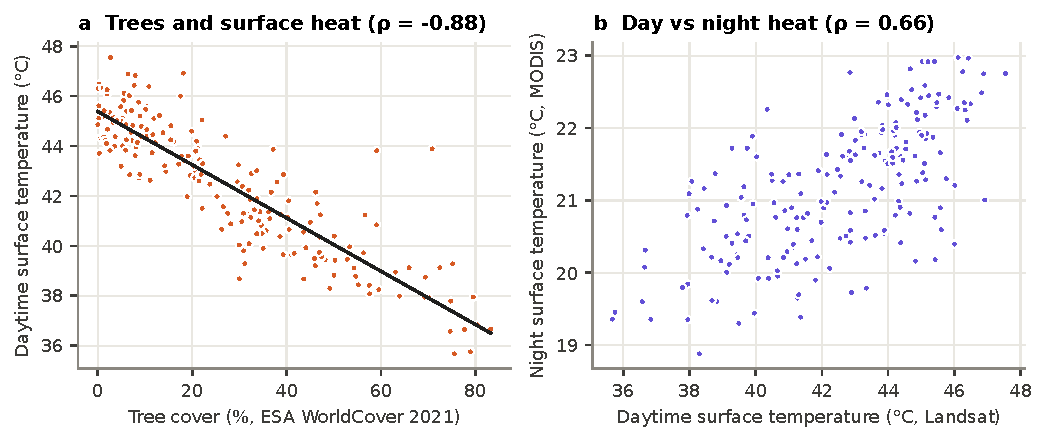
\includegraphics[width=\textwidth]{fig6_drivers.pdf}
\caption{(a) Tree cover and daytime surface temperature. (b) Daytime versus night-time surface temperature.}\label{fig:drivers}
\end{figure}

\begin{figure}[ht]\centering
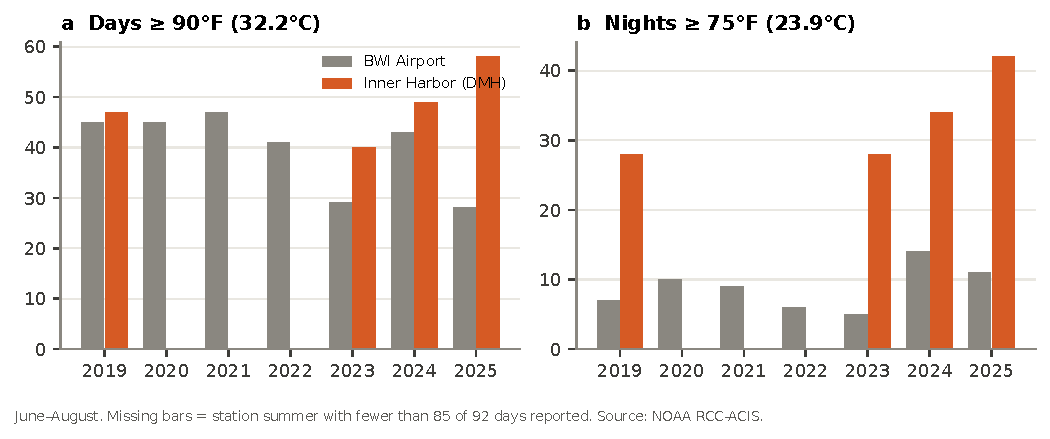
\includegraphics[width=\textwidth]{fig8_station_climate.pdf}
\caption{Hot days and warm nights at BWI airport and the Inner Harbor (DMH), June--August.}\label{fig:station}
\end{figure}

\begin{figure}[ht]\centering
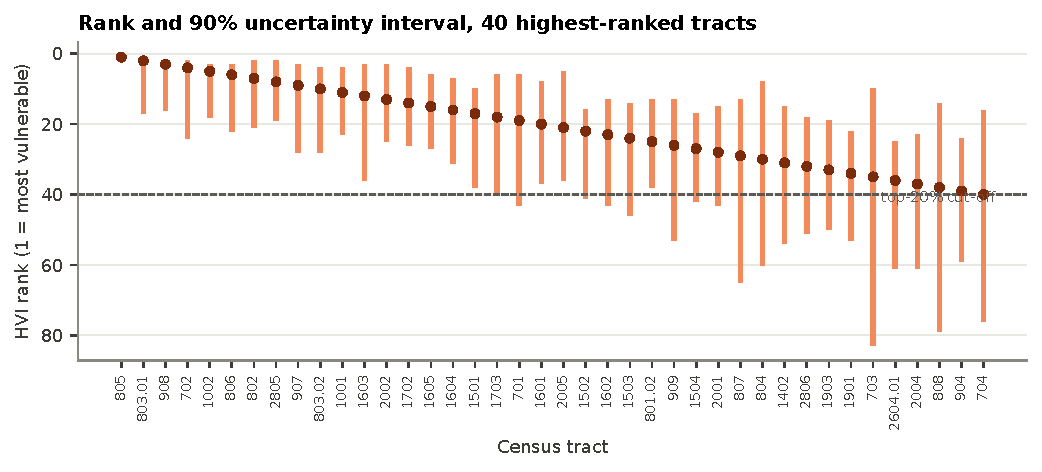
\includegraphics[width=\textwidth]{fig9_rank_uncertainty.pdf}
\caption{HVI rank and 90\% Monte Carlo interval for the 40 highest-ranked tracts.}\label{fig:rank}
\end{figure}

\end{document}
